\section{Implementation}

\begin{figure}[h]
    \centering
    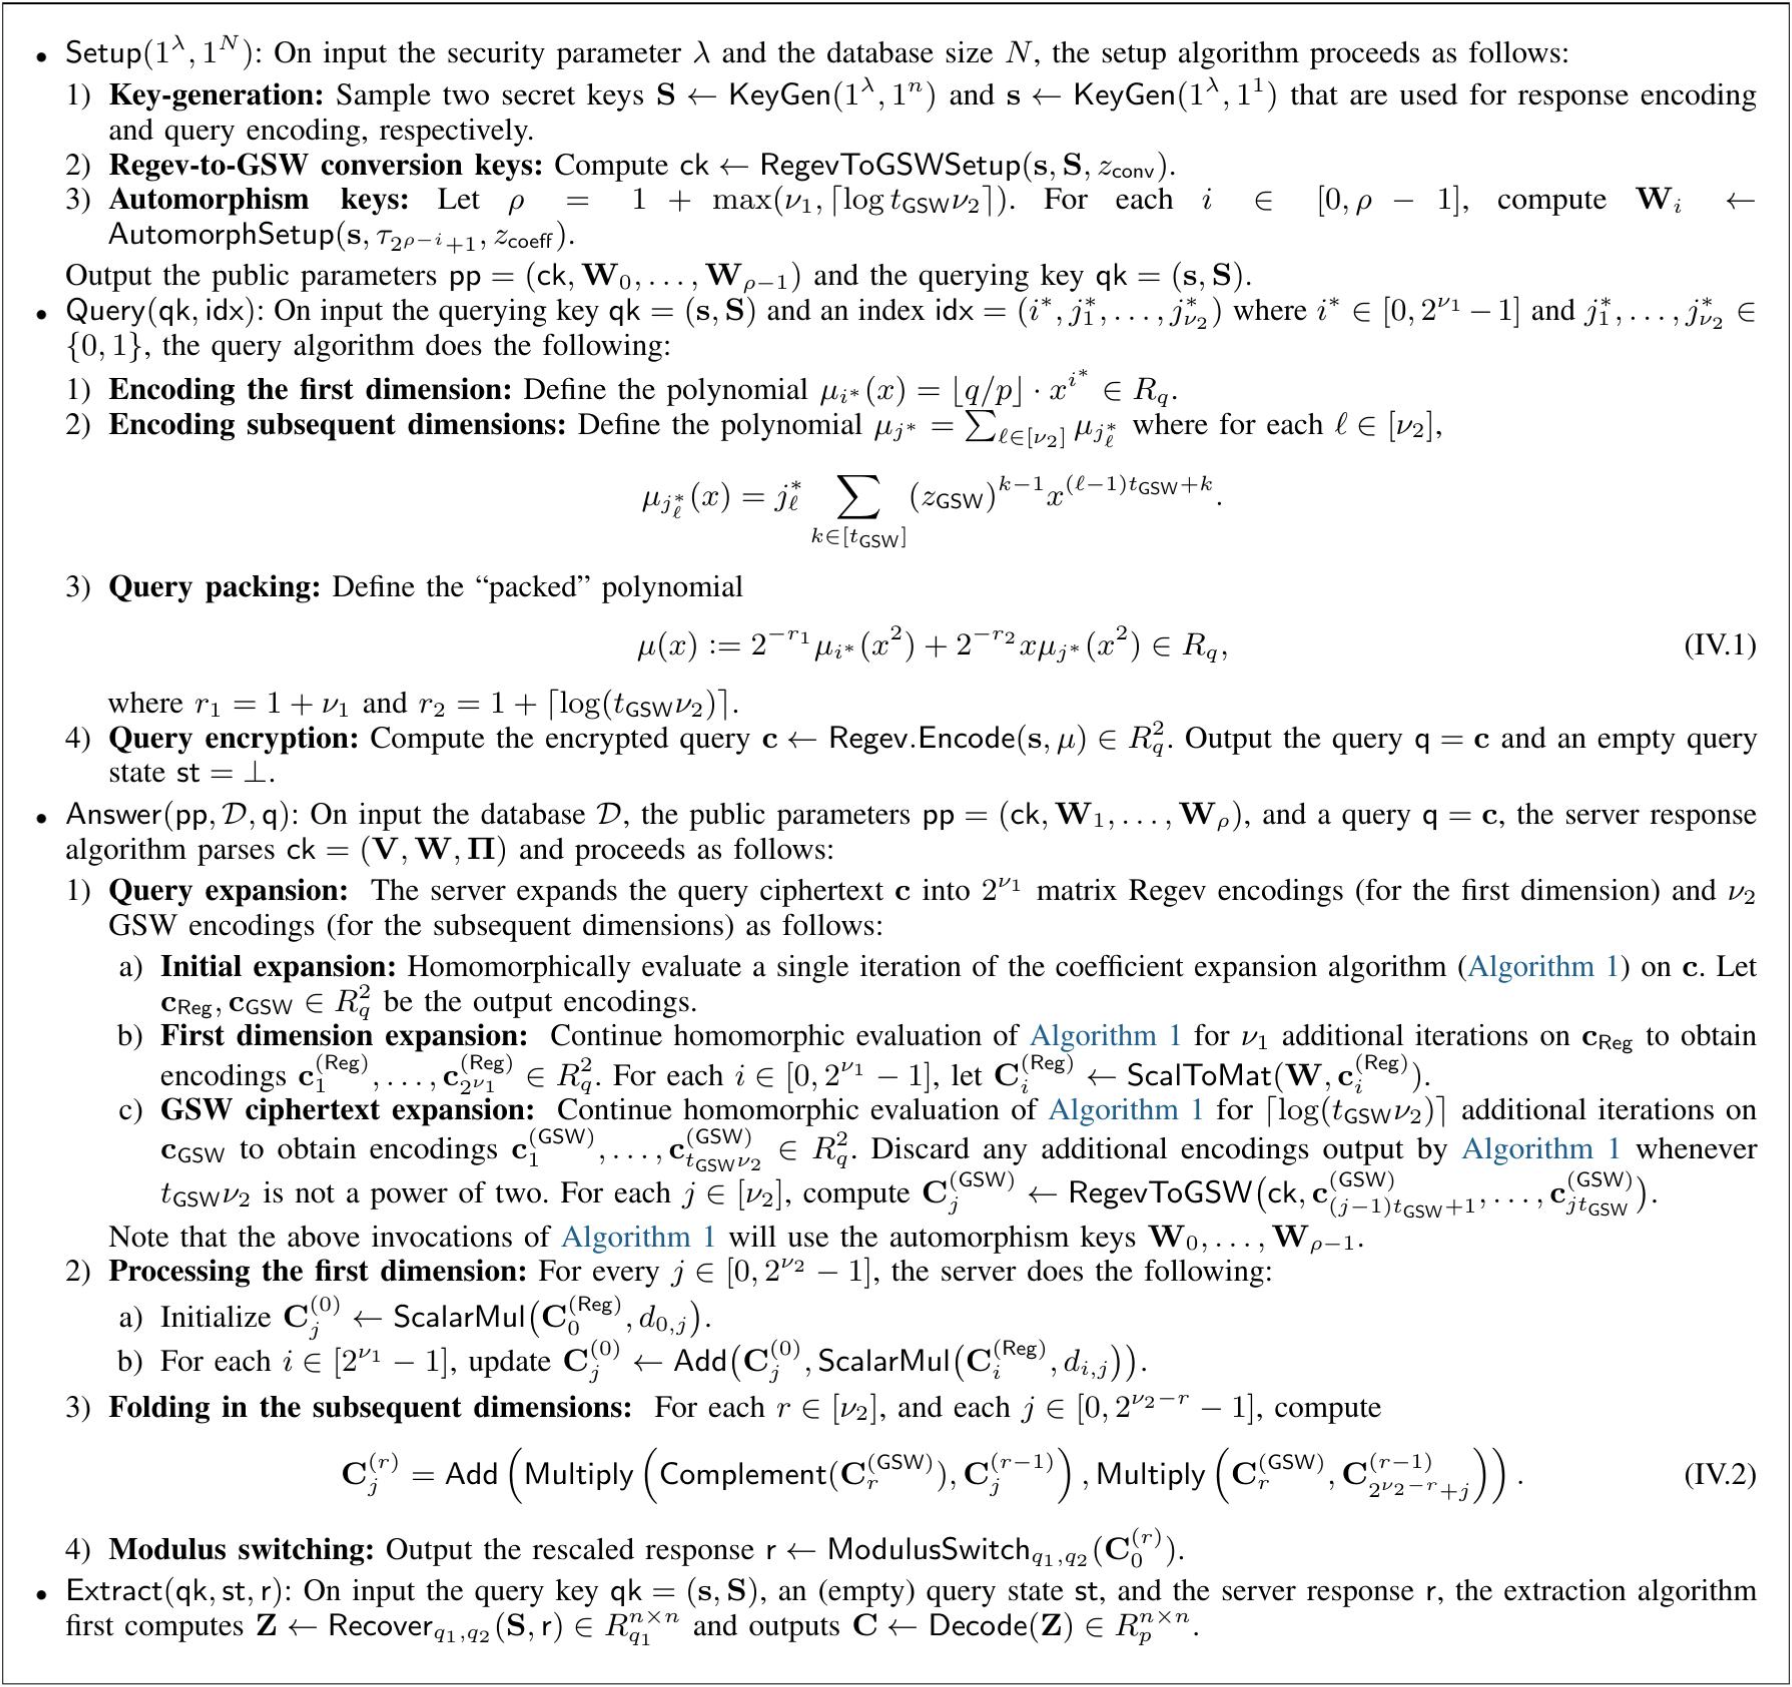
\includegraphics[width=\linewidth]{Images/Spiral_Protocol.png}
    \caption{The SPIRAL PIR protocol.}
    \label{fig:protocol_overview}
\end{figure}

In our architecture, we have seperated the Spiral codebase into individaul client and
server processes. Specifically, the client is repsonsible for the Setup
$\left(1^{\lambda}, 1^{N}\right)$, Query(qk, idx) and Extract(qk, st, r) stages of Fig.
\ref{fig:protocol_overview}, while the server is responsible for the Answer$(\mathrm{pp},
\mathcal{D}, \mathrm{q})$ process.

In addition to the above, we have extended the existing Spiral implementation to load in
a set of 32-byte hashes from a pre-defined database file. These set of hashes
may belong to a pre-defined sequence defined by the colouring or PBC procedure, and the hashes
are loaded by the order of insertion.

Furthermore, Spiral attempts to greatly reduce the size of the database by encoding
multiple hashes into a single database record. This results in faster query times while
lowering the overall in-memory storage requirement for the server. However, a consequence
to this approach results in the server sending back the requested hash nested other
existing hashes stored in the database. Therefore, the client maintains the ability to
\textit{extract} the queried hash from the received database record.

Likewise, the server attempts to compress as many hashes into every sequnetial record it
creates when building the database. A categorical explanation of these encoding methods
will be highlighted in the following sections.

In scenarios where the database size exceeds the number of hashes to load, the database is
padded with dummy polynomials, where every coefficient is set to zero. This is to ensure
database symmetry is maintained, and the server is able to perform matrix operations
across the database correctly.

\subsection{Encoding strategies}

Recall that a database record $d_{i}$ is an element of $R_{p}^{n \times n}$, where data is
encoded over the coefficients of a ring polynomial. The encoding strategy used to compress
multiple hashes across a single record is determined by the plaintext modulus $p$. The $p$ value is set
to be a power of two with a maximum value of $2^{30}$ and is selected during automatic
parameter selection\cite{1}.

The following table shows the relationship between a database size and the plaintext modulus $p$:

\begin{table}[h]
    \centering
    \begin{tabular}{|c|c|c|}
        \hline
        Database Size & Plaintext Modulus & Encoding Strategy \\
        \hline
        $2^{10}$ up to $2^{17}$ & 4   & Bucketing \\
        $2^{18}$ up to $2^{21}$ & 16  & Linear \\
        $2^{22}$ up to $2^{30}$ & 256 & Packing \\
        \hline
    \end{tabular}
    \caption{Relationship between database size and plaintext modulus.}
    \label{tab:encoding_strategies}
\end{table}

The following sections will briefly explain each strategy.

\subsubsection{Bucketing}

Bucketing is used when the maximum data representation provided by a single coefficent is
2 bits. Agian, this is used when $p$ is 4 and the value of a coefficient must wrap around the
plaintext modulus.

Bucketing involves storing a single hex charecter of a hash across multiple coefficients.
This will result in a \textit{bucket} of coefficients whichwill combinatorily represent a single
hex charecter as determined by a predefined lookup table. Given a hex contains 16
charecters, this lookup table is easily defined. The resulting encoding will be the length
of the input hash \times the number of coefficients in a bucket.

\subsubsection{Linear}

When $p$ is 16, we can directly represent a charecter in the value of a single
coefficient. The resulting encoding will be the length of the input hash.

\subsubsection{Packing}

Packing involves bit packing two charecters into a single coefficient when $p$ is 256. We
can use a 256 decimal value to binary pack two 4-bit integers. Note that a hexadecimal
charecter can be rpresented in 4 bits. This will resutl in an encoding that is half the
size of the input hash.
